% $File: report.tex
% $Date: Sat Dec 28 19:58:19 2013 +0800
% $Author: wyx <ppwwyyxxc@gmail.com>

\documentclass[11pt,a4paper]{article}

\usepackage{fontspec,amsmath,amssymb,zhspacing,verbatim,minted,listings,zhmath}
\usepackage{titlesec, titletoc}
\usepackage{enumerate}
\usepackage[hyperfootnotes=false,colorlinks,linkcolor=blue,anchorcolor=blue,citecolor=blue]{hyperref}
\usepackage[backend=biber]{biblatex}
%\usepackage[dvips]{graphicx}
\usepackage{subfigure}
\usepackage{indentfirst}
\usepackage{float}			% don't automatically change location of figure [H]
\usepackage{chngpage}		% use \changetext to change page size
\usepackage{caption}\captionsetup{hypcap=true}  % ref to jump to object instead of caption
\newfontfamily\zhfont[BoldFont=SimHei,ItalicFont=KaiTi_GB2312]{SimSun}
\lstset{keywordstyle=\color{blue!70}, commentstyle=\color{red!50!green!50!blue!50},frame=shadowbox,rulesepcolor=\color{red!20!green!20!blue!20},
basicstyle=\footnotesize\ttfamily}
\zhspacing
\setlength{\parindent}{2em}

\usepackage{fancyhdr}
\changetext{}{2.2cm}{-1.1cm}{-1.1cm}{}
\pagestyle{fancy}
\setlength{\headheight}{15.2pt}
\lhead[]{}\rhead[]{}
\fancyhead[C]{\emph{Image Stitching}}


%use cell in tabular
\newcommand{\tabincell}[2]{\begin{tabular}{@{}#1@{}}#2\end{tabular}}

%thick shline
\newlength\savewidth
\newcommand\shline{\noalign{\global\savewidth\arrayrulewidth\global\arrayrulewidth 1pt}
                   \hline
                   \noalign{\global\arrayrulewidth\savewidth}}


%\renewcommand{\abstractname}{摘要}
%\renewcommand{\contentsname}{目录}
%\renewcommand{\tablename}{表}
%\renewcommand{\figurename}{图}
\defbibheading{bibliography}{\section{References}}
\bibliography{refs.bib}
\newcommand{\figref}[1]{\hyperref[fig:#1]{Fig.\ref*{fig:#1}}}
\newcommand{\secref}[1]{\hyperref[sec:#1]{Sec.\ref*{sec:#1}}}
\newcommand{\tabref}[1]{\hyperref[tab:#1]{Tab.\ref*{tab:#1}}}

% math function
\let\Oldsum\sum
\renewcommand{\sum}{\displaystyle\Oldsum}
\let\Oldprod\prod
\renewcommand{\prod}{\displaystyle\Oldprod}


% $File: mint-defs.tex
% $Date: Fri Jan 06 14:25:30 2012 +0800
% $Author: wyx <ppwwyyxxc@gmail.com>


% \inputmintedConfigured[additional minted options]{lang}{file path}{
\newcommand{\inputmintedConfigured}[3][]{\inputminted[fontsize=\footnotesize,
	label=#3,linenos,frame=lines,framesep=0.8em,tabsize=4,#1]{#2}{#3}}

% \phpsrc[additional minted options]{file path}: show highlighted php source
\newcommand{\phpsrc}[2][]{\inputmintedConfigured[#1]{php}{#2}}
% \phpsrcpart[additional minted options]{file path}{first line}{last line}: show part of highlighted php source
\newcommand{\phpsrcpart}[4][]{\phpsrc[firstline=#3,firstnumber=#3,lastline=#4,#1]{#2}}
% \phpsrceg{example id}
\newcommand{\phpeg}[1]{\inputminted[startinline,
	firstline=2,lastline=2]{php}{res/php-src-eg/#1.php}}

\newcommand{\txtsrc}[2][]{\inputmintedConfigured[#1]{text}{#2}}
\newcommand{\txtsrcpart}[4][]{\txtsrc[firstline=#3,firstnumber=#3,lastline=#4,#1]{#2}}

\newcommand{\pysrc}[2][]{\inputmintedConfigured[#1]{py}{#2}}
\newcommand{\pysrcpart}[4][]{\pysrc[firstline=#3,firstnumber=#3,lastline=#4,#1]{#2}}

\newcommand{\confsrc}[2][]{\inputmintedConfigured[#1]{squidconf}{#2}}
\newcommand{\confsrcpart}[4][]{\confsrc[firstline=#3,firstnumber=#3,lastline=#4,#1]{#2}}

\newcommand{\cppsrc}[2][]{\inputmintedConfigured[#1]{cpp}{#2}}
\newcommand{\cppsrcpart}[4][]{\cppsrc[firstline=#3,firstnumber=#3,lastline=#4,#1]{#2}}


\begin{document}
%\fontsize{10pt}{\baselineskip}
%\selectfont
%\maketitle

%\begin{abstract}

	%{\bf 关键词}
%\end{abstract}
% File: title.tex
% Date: Sun Dec 29 00:15:06 2013 +0800
% Author: Yuxin Wu <ppwwyyxxc@gmail.com>

\newcommand{\HUGE}{\fontsize{29pt}{29pt}\selectfont}
\renewcommand{\today}{\number\year 年 \number\month 月 \number\day 日}
\begin{titlepage}

% 首行的位置往上调整。但vspace前面需要有东西才会起效。

\phantom{Start!}

\vspace{-1.7cm}

\begin{flushleft}

\emph{\Large Dept. of CST, Tsinghua University}\\[0.2cm]

\emph{\Large }\\[5.2cm]

% Title

\hspace{3cm}{ \HUGE \bfseries Image Retargeting}\\[0.4cm]


\hspace{3cm} {\huge \bfseries Project Report}

\end{flushleft}





\vfill



\begin{flushright}

{

%\setCJKmainfont{Adobe Kaiti Std}

% \pillar:使用一种统一的方法提高行高

\newcommand{\pillar}{ {\Huge \phantom{A}} }

\large

\begin{tabular}{lc}

\pillar Name & Yuxin Wu\\\cline{2-2}

\pillar Student No.& 2011011271 \\\cline{2-2}

\pillar Class  & CST-14 \\\cline{2-2}

\pillar Mail &ppwwyyxxc@gmail.com \\\cline{2-2}

\end{tabular}

}

\end{flushright}

\end{titlepage}

\tableofcontents
%\newpage

%\titleformat*{\section}{\centering\Large\bf}
% File: intro.tex
% Date: Fri Mar 28 00:14:44 2014 +0800
% Author: Yuxin Wu <ppwwyyxxc@gmail.com>
\section{Introduction}
This is an image retargeting program using Seam Carving\cite{sc} algorithm.

\subsection{Compilation}
Dependencies:

\begin{enumerate}
    \item gcc >= 4.7
    \item GNU make
    \item Magick++
\end{enumerate}

Compilation:
\begin{lstlisting}
$ make
\end{lstlisting}

\subsection{Run}
The program supports following command line arguments:
\begin{lstlisting}
  -i <file>   input image file
  -o <file>   output image file
  -w <num>   target width. can be the pixel number in integer, or a relative number in (0, 1]
  -h <num>   target height. same as above
  -e <file>   energy file, optional
  -m <file>   mask image, red to discard, green to keep. optional
  -c <type>   convolution type, can be one of 'prewitt', 'vsquare', 'sobel', 'laplacian'
  -p    use optimized seam carving.
  -f <file>   feature file. every line is a coordinate.
  -v    output intermidiate results to generate video demo.
\end{lstlisting}

\subsection{Examples}
\begin{enumerate}

  \item Output with every intermidiate result:

    \begin{lstlisting}
$ ./image_resize -i ./sea.png -o result.png -w 0.8 -v
$ feh path*.png
    \end{lstlisting}

    The original image and the result is as followed:

    \begin{figure}[H]
        \centering
        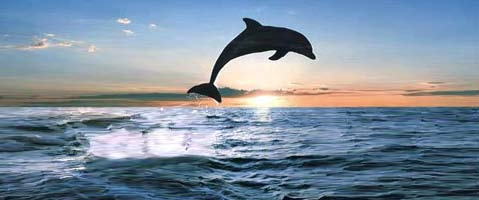
\includegraphics[width=0.9\textwidth]{src/sea.png}
    \end{figure}
    \begin{figure}[H]
        \centering
        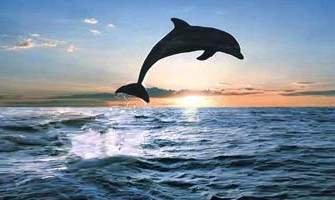
\includegraphics[width=0.63\textwidth]{result/sea.png}
    \end{figure}

  \item Use mask:
    \begin{lstlisting}
$ ./image_resize -i mike.jpg -o result.png -w 0.8 -m mike-m.png
    \end{lstlisting}
\end{enumerate}

% File: algo.tex
% Date: Mon Dec 30 23:27:10 2013 +0800
% Author: Yuxin Wu <ppwwyyxxc@gmail.com>

\section{Algorithms}

\subsection{Seam Carving}
This section will briefly introduce the main processes of Seam Carving algorithm
as well as the optimizaitons I made.
For the details of this algorithm, please refer to the original paper\cite{sc}.

\begin{enumerate}
    \item \textbf{Energy Map}

      An energy map of the original image must be first calculated to
      measue the ``importance'' of every pixel.
      In our implementation, four types of convolution kernel
      are supported to calculate energy map:

\begin{enumerate}
    \item Prewitt:
      \[ \begin{bmatrix}
          -1 & 0 & 1\\
          -1 & 0 & 1 \\
          -1 & 0 & 1\\
        \end{bmatrix} +
      \begin{bmatrix}
          -1 & -1 & -1\\
          0 & 0 & 0 \\
          1 & 1 & 1\\
        \end{bmatrix} \]

        \item vsquare
      \[ (\begin{bmatrix}
          -1 & 0 & 1\\
          -1 & 0 & 1 \\
          -1 & 0 & 1\\
        \end{bmatrix})^2 \]

      \item sobel(default)
      \[ \begin{bmatrix}
          -1 & 0 & 1\\
          -2 & 0 & 2 \\
          -1 & 0 & 1\\
        \end{bmatrix} +
      \begin{bmatrix}
          -1 & -2 & -1\\
          0 & 0 & 0 \\
          1 & 2 & 1\\
        \end{bmatrix} \]

      \item laplacian

        \[ \begin{bmatrix}
          -1 & 0 & -1\\
          0 & 4 & 0 \\
          -1 & 0 & -1\\
          \end{bmatrix}\]
\end{enumerate}

\item Mask
  The program allows users to use an image mask to declare the region they
  prefer to keep or discard. Users can modify the output energy grey image
  and adding red or green regions to it. Red region will have lower energy value,
  and therefore more likely to be discarded. Green region will be kept.

  \item Optimized Seam Carving

    \cite{sco} suggested an optimized version of seam-carving, by integrating seam-carving with scale.
    Their method first uses seam-carving to cut of certain number of seams,
    than apply a direct scale. They try all the possible number of seams to carve, and
    choose the best result measuring by their ``Patch-Level Image Dist Function'':

    \[ D(P, Q) = \sqrt{\sum_{i=1}^{nm}\sum_{j=1}^{nm}g_{ij}(p_i-q_i)(p_j-q_j)}\]

    Actually, from my observation, this formula is just a simple combination of the two factor: ``Coordinate Distance'' and
    ``Color distance'', measured by the two terms $g_{ij}$ and $(p_i-q_i)(p_j-q_j)$, respectively.

    There is a tradeoff between the two distance:
    if ``Color Distance'' is more important, the result tends to cut more seams and use less scaling.
    Since seam-carving can keep lots of patches in the image unchanged.
    If ``Coordinate Distance'' is more important, the algorithm is more likely to use scaling rather
    than seam-carving, since scaling keep the relative coordinate of every pixel unchanged.

    Therefore, the performace of this algorithm is strongly dependent on the choice of parameter,
    weighting the two types of distance mentioned above, i.e. the choice of $\sigma$ in $ g_{ij}$.
    From my experiements, it works well only when $\sigma$ is carefully selected. But most of the
    time the algorithm will only naively choose to use only seam-carving or only scaling.

    Also, this algorithm, although with parallel support, is still quite ineffective in computation,
    since the image distance takes too much time to calculate. One optimization can be made on
    the patch distance computation: I first assumed that all input image is needed for
    horizontally resize (since we can always transpose the image to get the same result).
    Then, when comparing a pair of patches,
    we can directly discard them if their vertical coordinate difference is larger than a threshold.
    This is reasonably because the ``Coordinate Distance'' mentioned above shall only
    account for horizontal coordinate distance.

  \item Feature Map

    I tried detecting keypoints in SIFT features, and add them to the energy map, since these are
    points that shall be kept. Keypoints coordinate will be Gaussian-blured before
    added to the energy map. However, this didn't give a better result than the original seam-carving,
    since SIFT keypoints are similar to those points previously detected by convolution.

\end{enumerate}


% File: result.tex
% Date: Mon Dec 30 23:50:29 2013 +0800
% Author: Yuxin Wu <ppwwyyxxc@gmail.com>

\section{More Results}
\begin{figure}[H]
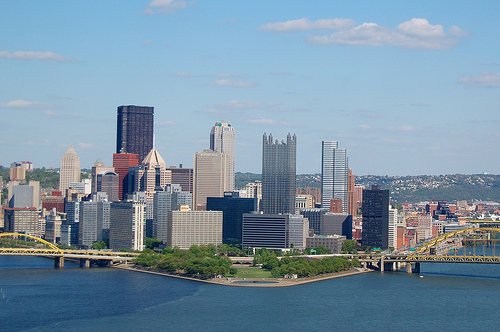
\includegraphics[height=8cm]{src/sea.jpg}\\
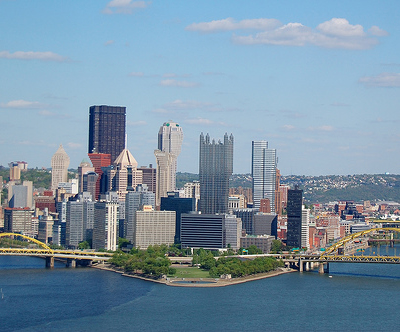
\includegraphics[height=8cm]{result/sea2.png}
\centering
\end{figure}

\begin{figure}[H]
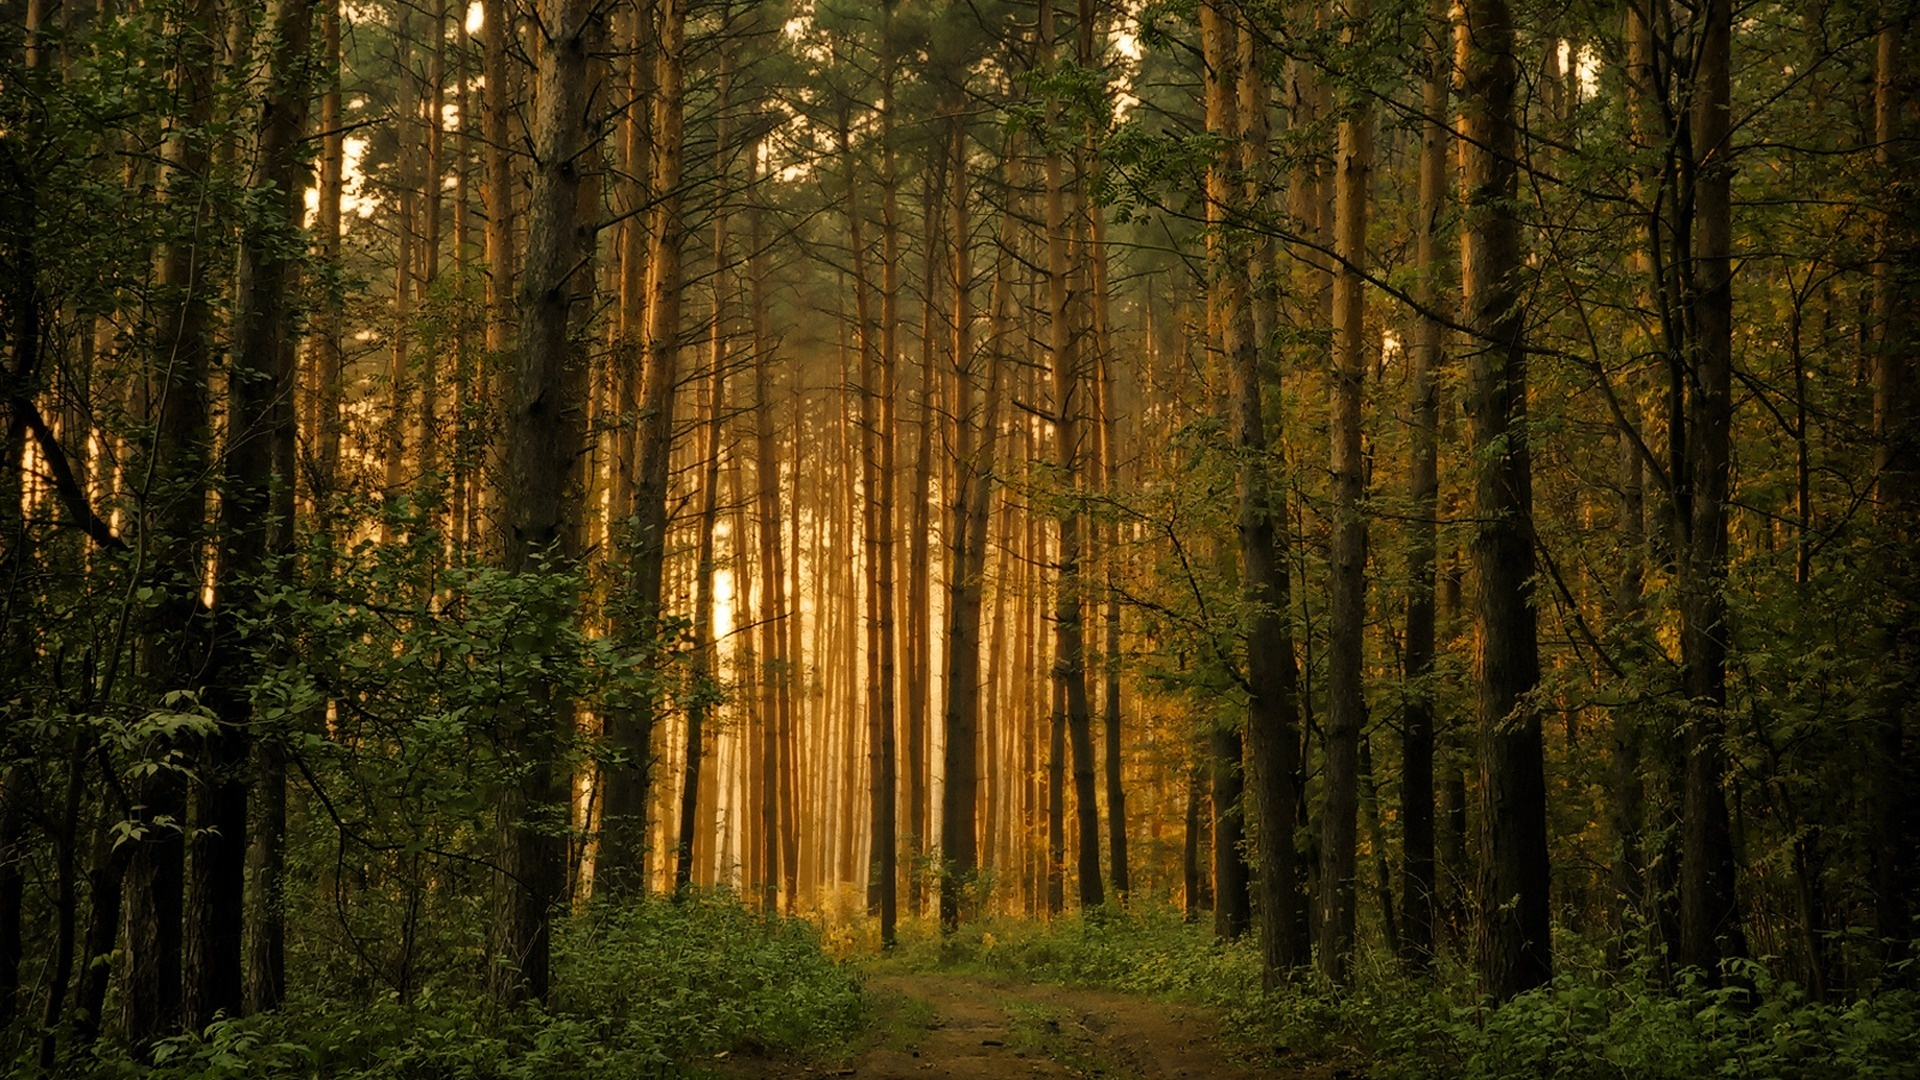
\includegraphics[height=8cm]{src/forest.jpg}\\
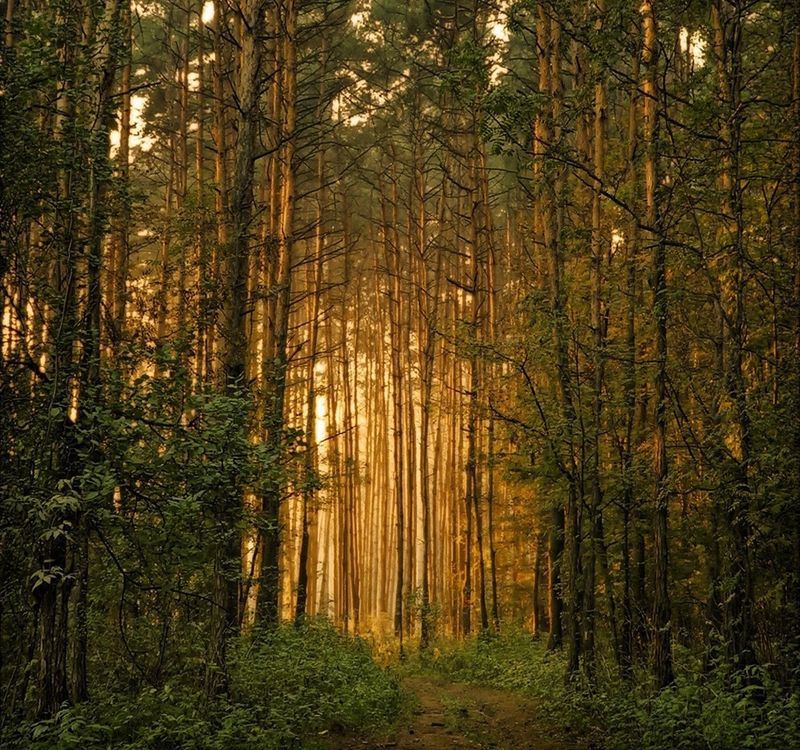
\includegraphics[height=8cm]{result/forest0.6.png}
\centering
\end{figure}

\begin{figure}[H]
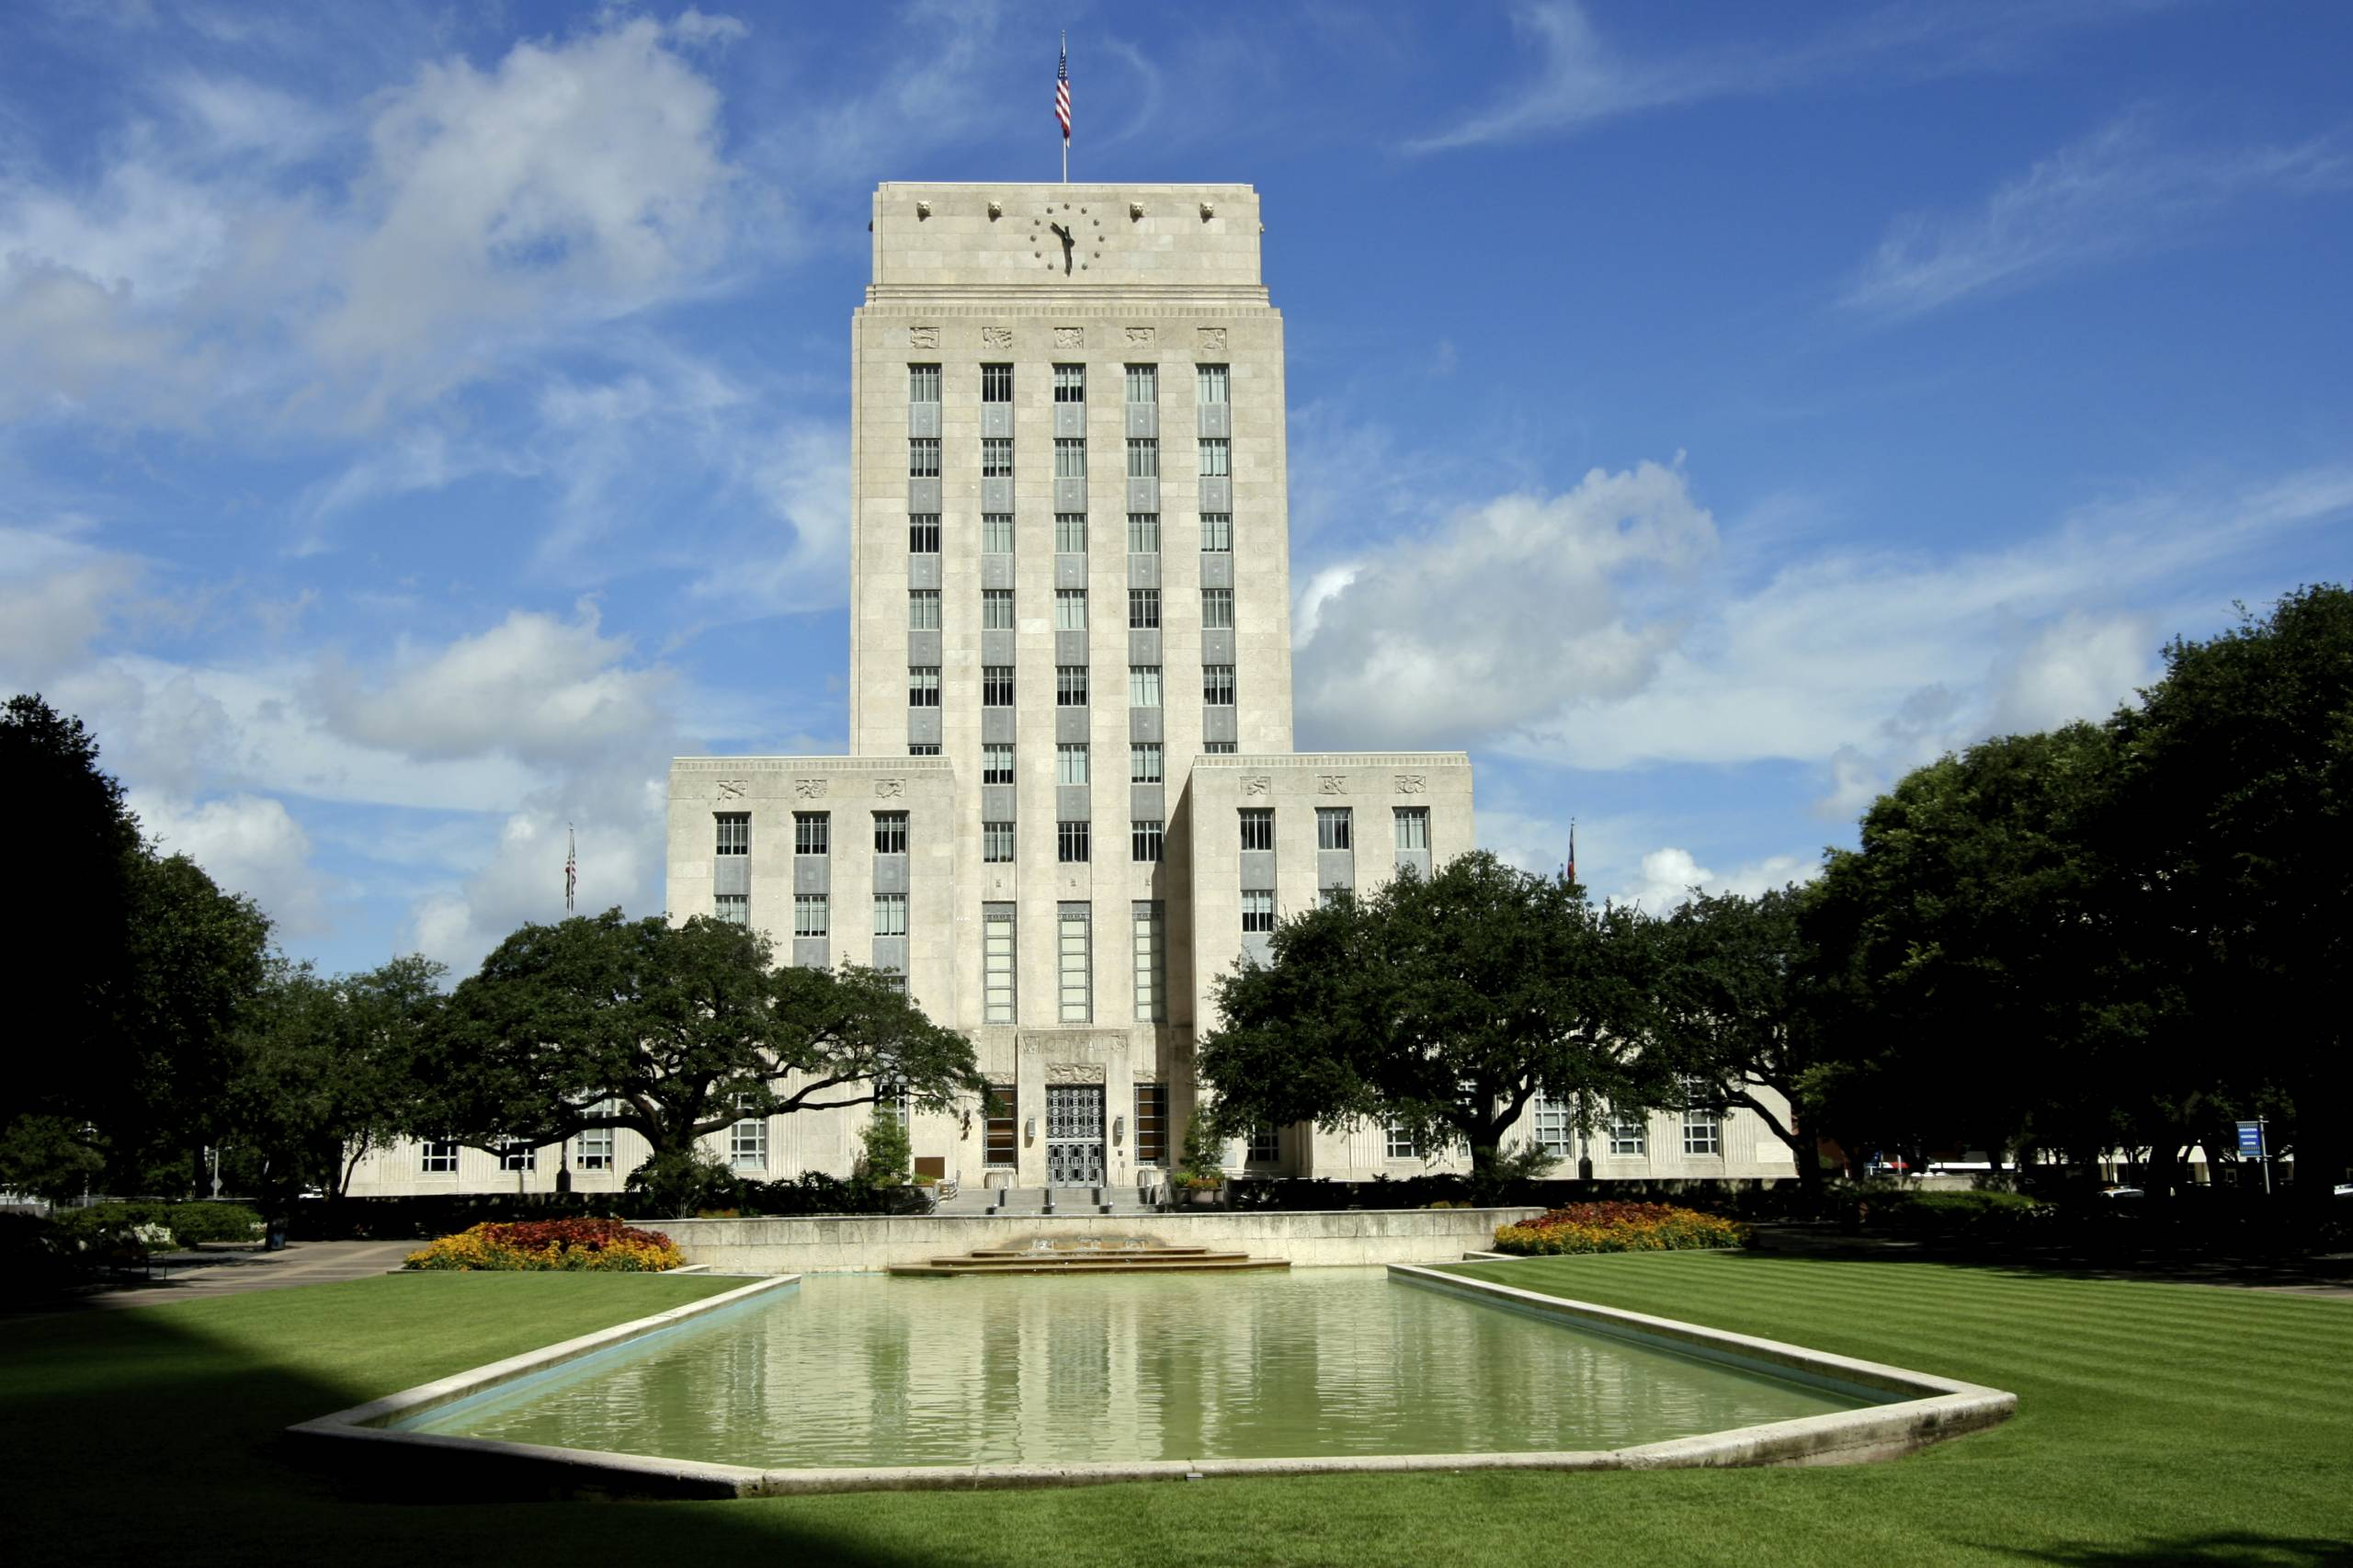
\includegraphics[height=8cm]{src/city.jpg}\\
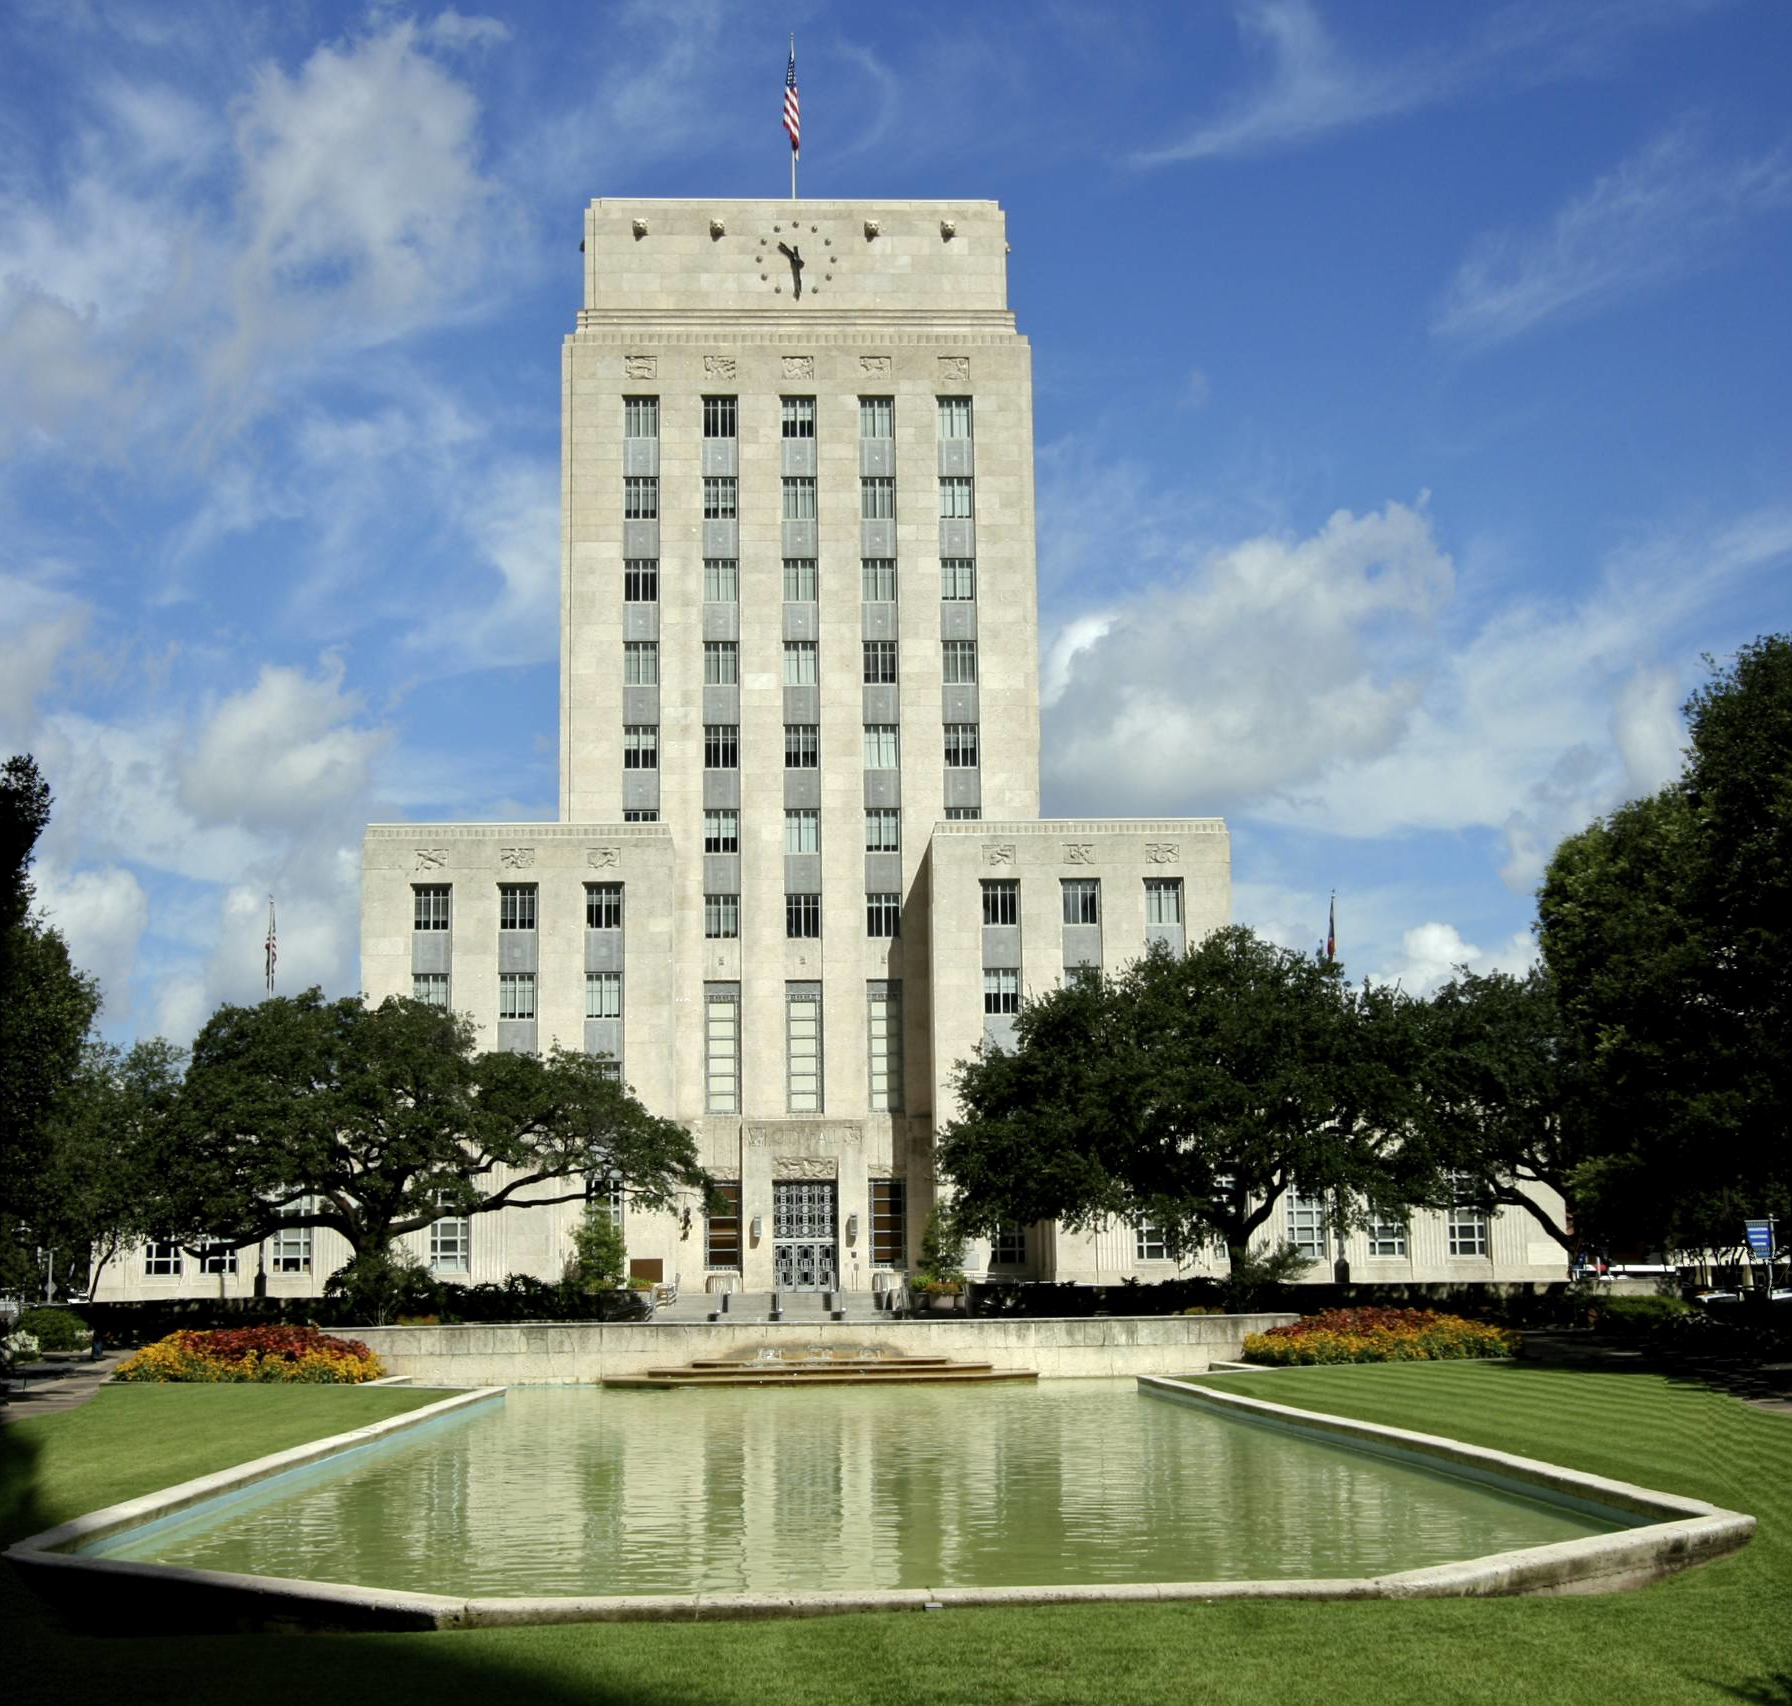
\includegraphics[height=8cm]{result/city.png}
\centering
\end{figure}

\printbibliography

\end{document}

